\section{Collective recurrence and geometric behavior}\label{sec:recurrence}
Paper~III studies two infinite families of towers in which the orbit returns, after a fixed number of steps, to a multiple of its starting point: for $G=5$ the period is $3$ steps with multiplier $4$ (\Src{III}{thm:R3T5c}), and for $G=11$ it is $8$ steps with multiplier $9$ (\Src{III}{thm:R3T5bp}). The Betti numbers of the corresponding complexes are known exactly for $k\le140$ (\Src{III}{thm:A5T6}) and eventually quasi-polynomial without an effective threshold (\Src{III}{thm:A5T53}). The \emph{scaling data} of a tower are the period, the multiplier, the value of $G$ and the growth law of $L_k$. The question here is whether the scaling data determine the topology.

\begin{proposition}[\SIV{8}: scaling information versus geometric structure]\label{prop:P8}\status{new; proved by exact computation on stated ranges (finite-exact)}
For $S_0\in\{126,3094\}$ and $x_k=(S_02^k)^2/5$ one has $C^3(x_k)=4x_k=x_{k+1}$, $L(x_k)=S_02^k$ and $G(x_k)=5$ for $0\le k\le11$ (twelve periods); the two towers therefore have the same \emph{normalized scaling signature} $\sigma=(G,\text{period},\text{multiplier},\rho)=(5,3,4,2)$, where $\rho=L(x_{k+1})/L(x_k)$ is the growth ratio of $L$. (The towers do \emph{not} share the values of $L$ itself: $L(x_0)=126$ and $3094$ respectively.) Their complexes $K(D(x_k))$ have, for each of $k=11,\dots,14$, Betti numbers $(1,6,5,0)$ for $S_0=126$ and $(1,10,9,1,0)$ for $S_0=3094$ (over $\mathbb F_2$). Hence the parameters $G$, the period, the multiplier and the growth ratio $\rho$ do not determine the Betti vector, even for $k$ in the stable range; in particular $\beta_3$ and the total Betti sum differ. No claim is made about any other scaling parameter, in particular about the initial value $L(x_0)$ or its divisor lattice.
\end{proposition}
\begin{proof}
Direct exact computation (Appendix~\ref{app:finite}): iterating $C$ on rationals for $36$ steps from $x_0$, comparing $C^{3j+3}(x_0)$ with $4C^{3j}(x_0)$ and computing $L$, $G$; and computing $K(D)$ and its $\mathbb F_2$-Betti numbers for $S_02^k$, $0\le k\le14$. For $S_0=126$ the values $(1,6,5,0)$ at $7\le k\le140$ are proved finite-exact in \Src{III}{thm:A5T6}; our computation agrees on $7\le k\le14$. The statement concerns only the stated ranges and makes no claim about larger $k$.
\end{proof}
\begin{remark}
The seeds are $126=2\cdot3^2\cdot7$ and $3094=2\cdot7\cdot13\cdot17$. The extra prime factors of $3094$ coincide with a non-zero $\beta_3$ although the modulus $5$, the period and the multiplier are identical. We do not identify which property of the divisor lattice of $S_0$ controls the Betti vector; that is the content of the open problem O5.
\end{remark}

\noindent\Cref{fig:scaling} shows $G=5$ scaling versus geometric evolution.

\begin{figure}[t]\centering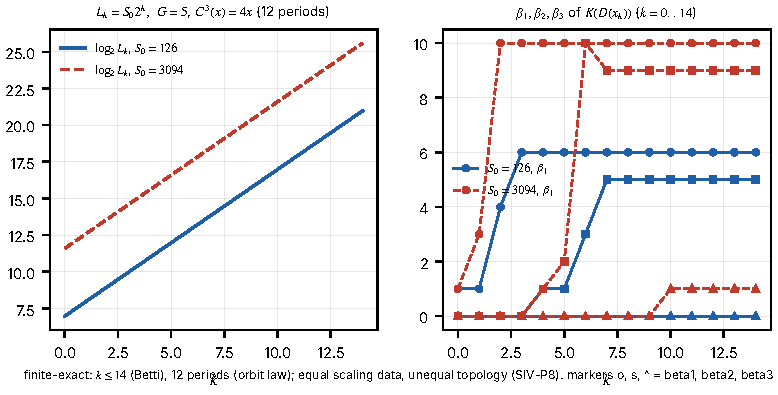
\includegraphics[width=\linewidth]{fig18_scaling_vs_topology.pdf}
\caption{\textbf{$G=5$ scaling versus geometric evolution.} Two towers with the same scaling signature $(G,\text{period},\text{multiplier},\rho)=(5,3,4,2)$ but different $L(x_0)$ (left) and different Betti numbers (right). \emph{Finite-exact: orbit law verified for twelve periods, Betti numbers for $0\le k\le14$; no extrapolation.}}\label{fig:scaling}\end{figure}
